\section{Poincar\'e Map}
\label{sec:Poincare}

\section{Periodic Orbits}
\label{sec:periodic}

Periodic orbit is a special type of trajectories, where its initial and final states are identical. Mathematically speaking, periodic orbits could be expressed in the following mannar:
\begin{equation}
\label{eq:periodicity}
x(t_0+T) = \Phi(t,x_0,T)x(t_0)
\end{equation}
where $x$ is the state vector, $T$ is called the period of the trajectory, $t_0$ is the initial time, and $x_0$ is the initial state. Equation \ref{eq:periodicity} illustrates that the given initial state and period, the state after a period $T$ should be the same as the initial state, hence the name periodic.

\section{Monodromy Matrix}
\label{sec:monodromy}
A linear mapping exists between the final state and initial state within a period, which is the $\Phi(t,x_0,T)$ matrix in equation \ref{eq:periodicity}. It has a official name as the Monodromy matrix. The idea of monodromy matrix is that it characterizes how perturbation in the initial state will propagate into the final state. So its eigenvalues indicate the stability of the dynamical system. When the eigenvalues lie within the unit circle in the complex plane, we could conclude that the system is stable, when the eigenvalues lie outside of the unit cirle, we could conclude that the system is unstable.

Note that monodromy matrix could not only be used to analyze periodic orbits, but also non-periodic dynamical systems. But when it was used to analyze periodic orbits, it is also known as the linearized Poincar\'e map.

\subsection{Monodromy Matrix for LTI system}

A Linear Time Invariant (LTI) system is one that evolves according to the following equations:
\begin{equation}
	\dot{x}(t) = Ax(t)+Bu(t)
\end{equation}
\begin{equation}
	y(t) = Cx(t)+Du(t)
\end{equation}
where A,B,C,D are constant matrices, x(t) is the evolving state, u(t) is the input vector and y(t) is the output of the system.
For a LTI system, the state transition matrix is:
\begin{equation}
	\Phi(t,t_0) = e^{A(t-t_0)}
\end{equation}



\begin{comment}

A sequential and iterative design process was adopted to refine simulation model and mechanical design as shown in Figure \ref{fig:systemOverview}. The 1-DOF template \cite{Full1999} called \textbf{knee extensor model} was used to investigate the torque and angular speed requirement of the leg, as depicted in Figure \ref{fig:systemOverview}(a). It assumes all masses are lumped at the base; thigh and shank link are of same length and have no mass or inertia; foot is located directly below the hip, which means no horizontal off-set for foot hold. Jumping motion was simulated using this knee extensor model under various motors' maximal speed and maximal torque. These simulations in turn exposed the speed and torque requirements in order to achieve the desired motion, which provides guidance for choosing appropriate motor and gear ratio.

A more detailed leg model with motors' rotary inertia and horizontal foot off-set was introduced as shown in Figure \ref{fig:systemOverview} (b). The detailed leg model was used to further narrow the choice of gear ratio by minimizing ground impact force while maintaining balance between torque and speed requirements. Optimized parameters were tested on the hardware platform shown in Figure \ref{fig:systemOverview} (c) to validate the design.

\begin{figure}
	\centering
	\resizebox{1.0\linewidth}{!}{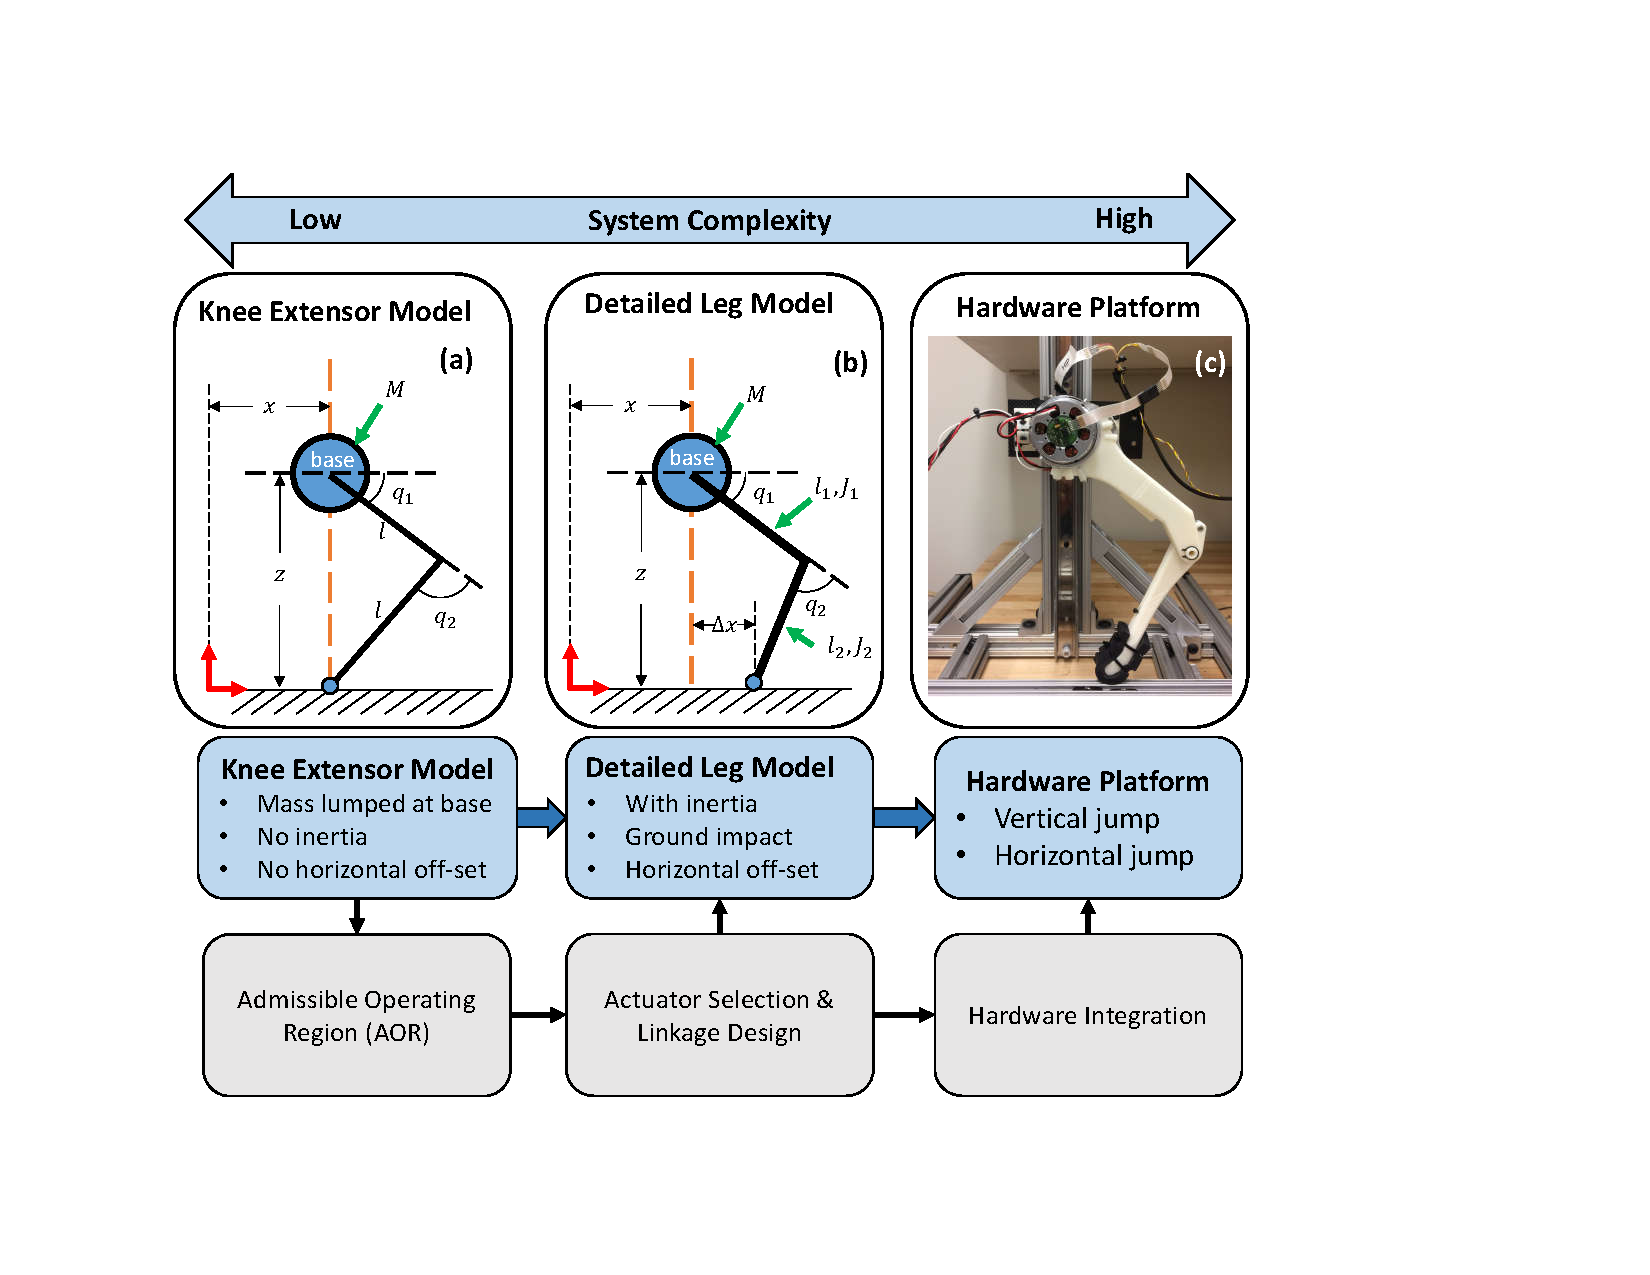
\includegraphics{system_overview.pdf}}
	\caption{Sequential design process for determining design parameters. (a) knee extensor model for motor selection (b) detailed leg model for linkage design and gear ratio choice (c) hardware platform for experiments}
	\label{fig:systemOverview}
\end{figure}

%-------------------------------------------
% ----------Knee Extensor Model----------
\subsection{Knee Extensor Model}
\label{sec:kneeExtensorModel}

The knee extensor model was used to estimate the torque and speed requirements to achieve desirable jumping motions, which provides us with an initial guidance for choosing motor and gearbox. Figure \ref{fig:systemOverview} (a) shows the schematics of the knee extensor model. The model assumes that all masses are lumped at the base to be $M$, which is mounted on a vertical linear rail. Thigh and shank links have an identical length of $l$, while its foot and base are vertically aligned. Hence only the knee joint needs to be actuated to perform vertical jump while the hip joint is not actuated. The vertical height of the base $z$ and joint angles $q_1, q_2$ are shown in Figure \ref{fig:systemOverview}.

The dynamics of this model was formalized as a single point mass accelerated due to ground reaction force (GRF). Ground reaction force was chosen as the control input because it is the only external force in the knee extensor model that could increase the mechanical energy of the system. The equation of motion (EOM) of the system is: $\ddz = \frac{F_z}{M}-g$, where $z$ is the vertical displacement of the base, $F_z$ is the vertical component of GRF, $M$ is the lumped mass at the base and $g$ is the gravitational acceleration. 

%-------------------------------------------
% ----------GRF Parameterized as \Bezier\ Polynomial----------
\subsection{GRF Parameterized as \Bezier\ Polynomial}
\label{sec:BezierPoly}
	
A $5^{th}$ order \Bezier\ polynomial was used to parameterize the GRF profile. The reasons for using \Bezier\ Polynomial to parametrize the ground reaction force is two fold. Firstly, the first and last coefficient of a \Bezier\ polynomial corresponds to the initial and final value of the GRF, which makes it more convenient to anchor GRF to desired values at the initial and final instance; secondly, integration of \Bezier\ Polynomial is a linear operation, which is computationally inexpensive. This property is utilized in integrating the prescribed ground reaction force and integrate to get the velocity trajectory, as shown in Equation \ref{eq:bernstein_integration}, and integrate again to get the position trajectory

The coefficients of \Bezier\ polynomial are assumed to be $[Mg, \alpha_1, \alpha_2, \alpha_3, \alpha_4, 0]$. The first coefficient was set to be the weight of the leg because it is assumed that the leg starts from static equilibrium state, and last coefficient was set as $0$ to ensure a smooth and physically feasible motion at the take-off moment.  

The Bernstein polynomials are defined over [0,1] as:

\begin{equation}
	B_{i,N} = \left(
	\begin{smallmatrix}
	N\\
	i
	\end{smallmatrix}\right)
	x^i(1-x)^{n-i},
	0\leq i \leq N
\end{equation}
where  $\left(
\begin{smallmatrix}
N\\
i
\end{smallmatrix}\right)$
is the binomial coefficients.

Since a \Bezier\ polynomial is the linear combination of a Bernstein polynomial basis\cite{dicsibuyuk2007generalization} defined as,

\begin{equation}\label{eq:bezier}
C_N(s) = \sum_{i=0}^{N}\alpha_i B_{i,N}(s)
\end{equation}

where $\alpha_i$ is the coefficient for the $i^{th}$ Bernstein polynomial $B_{i,N}$, analytical solution for velocity and position could be obtained using the property of the Bernstein polynomial\cite{Doha2011}:

\begin{equation} \label{eq:bernstein_diff}
\frac{d}{ds}B_{i,N}(s)=\frac{N}{T}(B_{i-1,N-1}(s)-B_{i,N-1}(s))
\end{equation}
where $s$ is a point between general time interval $[0, T]$.

Given the initial velocity $\dz_0$, the velocity trajectory in stance phase is a $6^{th}$ order \Bezier\ polynomial with coefficients $\gamma_{(0-6)}$. The linear relationship between force and velocity \Bezier\ coefficient is:

\begin{equation}\label{eq:bernstein_integration}
\frac{6}{T_{st}}\left[
\begin{smallmatrix}
-1 & 1 & 0 & 0 & 0 & 0 & 0 \\
0 &-1 & 1 & 0 & 0 & 0 & 0 \\
0 & 0 &-1 & 1 & 0 & 0 & 0 \\
0 & 0 & 0 &-1 & 1 & 0 & 0 \\
0 & 0 & 0 & 0 &-1 & 1 & 0 \\
0 & 0 & 0 & 0 & 0 &-1 & 1 \\
1 & 0 & 0 & 0 & 0 & 0 & 0 \\
\end{smallmatrix}
\right]
\left[
\begin{matrix}
\gamma_0\\\gamma_1\\\gamma_2\\\gamma_3\\\gamma_4\\\gamma_5\\\gamma_6\\
\end{matrix}
\right]
=
\left[
\begin{matrix}
\left[
\begin{matrix}
0\\\alpha_1\\\alpha_2\\\alpha_3\\\alpha_4\\0\\
\end{matrix}
\right]\frac{1}{M}-g\\
\dz_0\\
\end{matrix}
\right]
\end{equation}
where $T_{st}$ is the stance duration for jumping up.

Similarly, the position trajectory in stance phase could also be integrated by applying the linear operation shown in Equation \ref{eq:bernstein_integration} given initial position $z_0$. At each instance  $t\in[0,T_{st} ]$, the joint angle $q=[q_1,q_2]$ defined in Figure \ref{fig:systemOverview}(a) was solved by inverse kinematics. 

Since the thigh and shank links are assumed to be massless, joint torque $\tau=[\tau_1,\tau_2]$ could be reconstructed using 
\begin{equation}
	\tau=J(q)^T F
\end{equation}

where $\tau_1$ and $\tau_2$ are joint torques for hip and knee joints, $F$ is the ground reaction force, and $J(q)\in R^{2\times 2} $ is the manipulator Jacobian of the foot relative to the hip.

The jumping performance was evaluated by the maximal reachable height $h_{max}$,
 \begin{equation}
 	 h_{max} := h_{to}+\frac{v_{to}^2}{2g}
 \end{equation}

 where $h_{to}$ and $v_{to}$ are the base height and speed at the moment of take-off.

%---------------------------------------------------------------------
% ----------Nonlinear Optimization for Ground Reaction Force----------
\subsection{Nonlinear Optimization for Ground Reaction Force}
\label{sec:nonlOptGRF}

In order to get the optimal ground reaction force profile within actuator limits, an optimal control problem was formulated and solved using nonlinear optimization:
\begin{equation}\label{eq:path_constraints}
\begin{aligned}
\min&~~~~~~~~~~-h_{max}\\
s.t.&~~~~~~~q_{lb}\leq q \leq q_{ub}\\
&~~~~~~~\dq_{lb}\leq \dq \leq \dq_{ub}\\
&~~~~~~~\tau_{lb}\leq \tau \leq \tau_{ub}\\			 	
\end{aligned}
\end{equation}
where $q_{lb}$, $q_{ub}$ are the lower and upper bounds for joint angles; $\dq_{lb}$, $\dq_{ub}$ for angular velocity; $\tau_{lb}$, $\tau_{ub}$ for joint torques.  

Dynamics was discretized at $N$ sampling points to search for optimal variable values. Joint angle $q$ and angular velocity $\dq$ were discretized at the sampling points. Motor's maximal speed and torque constraints were imposed at each sampling point as inequality constraints.

The optimization variables are chosen as follows:
\begin{equation}\label{eq:opt_var_knee}
x_{opt} = [z_0, \alpha_{(1-4)}, T_{st}, q_{(1-N)}, \dq_{(1-N)}]
\end{equation}
where $x_{opt}$ is the vector of optimization variables for stance phase; $z_0$ is the base's vertical initial position; $\alpha_{(1-4)}$ are the \Bezier\ polynomial coefficients of ground reaction force; $T_{st}$ is the total stance time; $q$ is the vector of joint angles and $\dq$ is the vector of joint velocities at all the sampling points.

Equality constraints were imposed to satisfy forward kinematics:

\begin{equation}
\label{eq:kin_position}
rot(q_1)
\left[\begin{matrix}
l\\0
\end{matrix}\right]
+
rot(q_1+q_2)\left[\begin{matrix}
l\\0
\end{matrix}\right]
+
\left[\begin{matrix}
0\\z
\end{matrix}\right]
=0
\end{equation}

\begin{equation}
\label{eq:kin_velocity}
J(q)\dq+\left[\begin{matrix}
0\\ \dz
\end{matrix}
\right]
=
\left[\begin{matrix}
0\\0
\end{matrix}\right]
\end{equation}
where $rot\in SO(2)$ is the rotation matrix. $z$ and $\dz$ are the vectors of height and velocity of the base at each sampling point using Equation \ref{eq:bernstein_integration}.


MATLAB's $fmincon$ function was used to search for local optimal solutions. The parameters for the knee extensor model is chosen as follows: mass $M = 0.66~kg$, link length $l=0.12~m$. 100 simulation runs were executed over 10 different maximal motor speed ($\omega_{max}$ from 23 rad/s to 37 rad/s) and maximal torque ($\tau_max$ from 6.2 Nm to 9.7 Nm) constraints, then the maximal achievable height $h_{max}$ is plotted as the third axis against $\tau_{max}$ and $\omega_{max}$. As shown in Figure \ref{fig:hmax_pcolor}, the maximal achievable height increases as the upper limit for speed and torque increases. The level curves shows that $h_{max}$ could reach as high as 0.8 m theoretically with the effective actuator torque of 9.7 Nm and actuator speed of 37 rad/s.

The advantage of this method is that it decoupled the study of jumping to two decoupled problems. In terms of dynamics, it treats the leg as a point mass accelerated due to ground reaction force and gravity; in terms of kinematics, it assumes two link kinematics chain for leg topology. After imposing equality constraints which bridges the error between kinematics as shown in Equations \ref{eq:kin_position} and Equation \ref{eq:kin_velocity}, the problem is tackled in a way that avoids the problem of singularity in the search of optimization variables.


%-----------------------------------------------
% ----------Admissble Operating Region----------
\subsection{Admissble Operating Region}
\label{sec:AOR}

\begin{figure}
	\centering
	\resizebox{1.0\linewidth}{!}{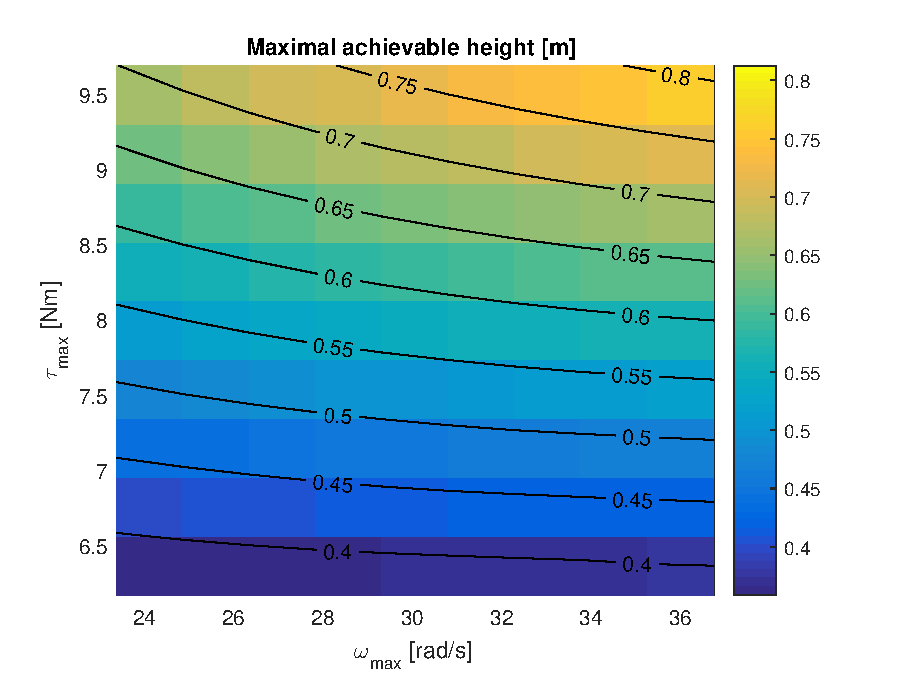
\includegraphics{hmax_pcolor.eps}}
	\caption{Maximal achievable height for specific torque and speed limit. The x-axis corresponds to maximal angular velocity of the actuator, the y-axis corresponds to maximal torque of the actuator, and the depth represents the maximal achievable height of a jump}
	\label{fig:hmax_pcolor}
\end{figure}

\begin{figure}
	\centering
	\resizebox{0.8\linewidth}{!}{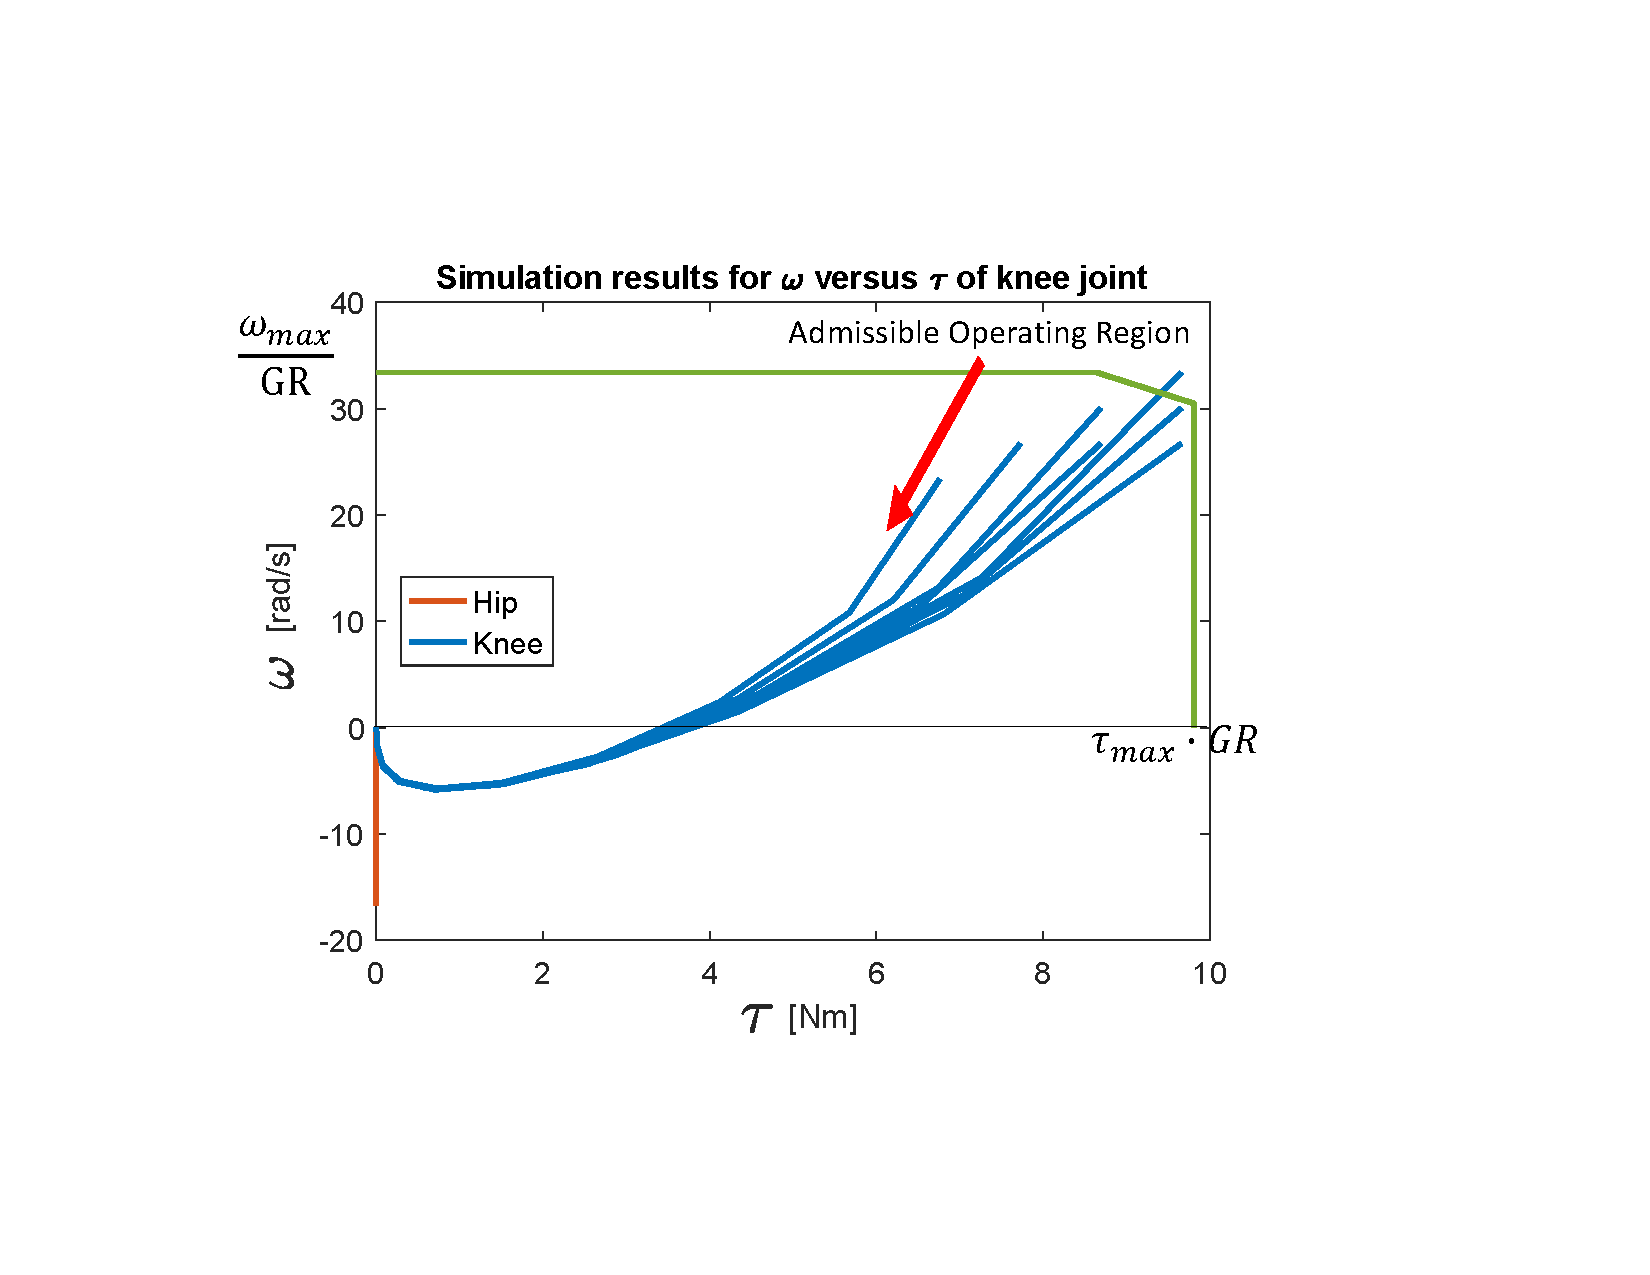
\includegraphics{AOR.pdf}}
	\caption{The Admissible Operating Region (AOR) formed by the torque and angular speed trajectories from the one hundred knee extensor model simulations. A typical motor's speed-torque curve scaled by gear ratio of 23:1 is plotted in green curve. Hip motor acts as a passive joint throughout the jumping up phase.}
	\label{fig:AOR}
\end{figure}

 In general, Admissible Operating Region (AOR) is defined as the area in the torque-speed plane enclosed by the Leg's torque-speed trajectory in performing certain task, as is shown in Figure \ref{fig:AOR}. The motions corresponding to the enclosed AOR region are admissible to the actuator. It is a projection of dynamic motion to the torque-speed domain of the actuators. It is a lumped quantity which treats the motor and gearbox as a unity instead of separating the characteristics of both. The contribution of the proposition of AOR is that it captures the essence of robot motion generation, and bridges between motor dynamics, and workspace dynamics. Furthermore, it could be used in the early stage of design by projecting workspace dynamics to actuator's speed-torque space, before the choice of motor and transmission design is determined. 
 
 \subsubsection{Scaling Effect of Gear Ratio}
 \label{sec:GR_scale_effect}
 
 The analysis of AOR takes motor and gearbox as a whole entity. Since AOR is determined by desired motion, it does not change with gear ratio, hence it is independent of actuator and gearbox choices. What the gear ratio could scale is the motor characteristic curve. Shown as the green curve in Figure \ref{fig:AOR}, the original speed-torque curve of this specific motor is scaled by gear ratio to enclose more of the AOR. Namely, the maximal motor speed $\omega_{max}$ is scaled down to $\omega_{max}/GR$, and the maximal motor torque $\tau_{max}$ is multiplied to $\tau_{amx}GR$. Geometrically speaking, the motor characteristic curve has become lower and wider. 
 
 \subsubsection{Zero Torque at the Hip Joint}
 
 Multiple simulation results from Section \ref{sec:nonlOptGRF} is plotted in Figure \ref{fig:AOR} shown as blue curves. Note that the torque requirement for Hip motor shown in red line is always zero. This result conforms to our formulation of the Knee Extensor Model, which assumes the foot is located directly below the hip point.
 
 \end{comment}
 
 

